\documentclass{scrreprt}

\usepackage{amsmath}
\usepackage{amsthm}
\usepackage{amssymb}
\usepackage{bm}
\usepackage[shortlabels]{enumitem}
\usepackage{framed}
\usepackage{hyperref}
\usepackage[utf8]{inputenc}
\usepackage{multicol}
\usepackage{mathtools}
\usepackage{physics}
\usepackage{polynom}
\usepackage{tabularx}
\usepackage[table]{xcolor}
\usepackage{titling}
\usepackage{fancyhdr}
\usepackage{xfrac}
\usepackage{pgfplots}

\pgfplotsset{compat = newest}
\usepgfplotslibrary{fillbetween}
\usetikzlibrary{patterns}
\usetikzlibrary{through}


\author{Karsten Lehmann}
\date{WiSe 2024/25}
\title{Übungsblatt 1\\INF-B-110, Lineare Algebra}

\setlength{\headheight}{26pt}
\pagestyle{fancy}
\fancyhf{}
\lhead{\thetitle}
\rhead{\theauthor}
\lfoot{\thedate}
\rfoot{Seite \thepage}

\begin{document}
\paragraph{Ü1.3 Rechnen mit komplexen Zahlen}
Ermitteln Sie für die komplexen Zahlen
\[
  z_1 = 1 + i, \qquad
  z_2 = 2i, \qquad
  z_3 = \sqrt{8}e^{i \cdot \frac{3}{4}\pi}, \qquad
  z_4 = \sqrt{12}\qty(\cos\frac{4}{3}\pi + i\sin\frac{4}{3}\pi)
\]
jeweils arithmetische, trigonometrische und Eulersche Darstellung.
Berechnen Sie die komplexen Zahlen
\[
  z_2 + z_3, \qquad
  z_1 \cdot z_3, \qquad
  \frac{z_3}{z_1}, \qquad
  \overline{z_4}, \qquad
  \abs{z_1^2}, \qquad
  \frac{1}{2}\qty(z_3 + \overline{z_3}), \qquad
  \frac{i}{2}\qty(z_4 - \overline{z_4})
\]
und geben Sie sie in arithmetischer Darstellung an.

\subparagraph{Lsg.}
\textbf{Arithmetische Darstellung:}
\begin{enumerate}[(1)]
\item $z_1 = 1 + i$
\item $z_2 = 2i$
\item $z_3 = \sqrt{8} \cdot \cos\qty(\frac{3}{4}\pi) +
  \sqrt{8} \cdot \sin\qty(\frac{3}{4}\pi) \cdot i =
  -\frac{\sqrt{8}}{\sqrt{2}} + \frac{\sqrt{8}}{\sqrt{2}} \cdot i
  = - \sqrt{\frac{8}{2}} + \sqrt{\frac{8}{2}} \cdot i
  = -2 + 2 \cdot i$
\item $z_4 = \sqrt{12} \cdot \cos\qty(\frac{4}{3}\pi) +
  \sqrt{12} \cdot \sin\qty(\frac{4}{3}\pi) \cdot i =
  -\frac{\sqrt{12}}{2} - \frac{\sqrt{12} \cdot \sqrt{3}}{2} \cdot i
  = -\sqrt{3} - 3 \cdot i$
\end{enumerate}
\textbf{Trigonometrische Darstellung:}
\begin{enumerate}[(1)]
\item
  \begin{flalign*}
    z_1 &= \abs{\sqrt{1^2 + 1^2}} \qty(
      \cos\qty(\cos^{-1}\qty(\frac{1}{\abs{\sqrt{1^2 + 1^2}}})) +
      \sin\qty(\sin^{-1}\qty(\frac{1}{\abs{\sqrt{1^2 + 1^2}}})) \cdot i
     ) & \\
        &= \sqrt{2} \qty(\cos\qty(\frac{\pi}{4}) + \sin\qty(\frac{\pi}{4}) \cdot i)
  \end{flalign*}
\item
  \begin{flalign*}
    z_2 &= \abs{\sqrt{0^2 + 2^2}} \qty(
      \cos\qty(\cos^{-1}\qty(\frac{0}{\abs{\sqrt{0^2 + 2^2}}})) +
      \sin\qty(\sin^{-1}\qty(\frac{2}{\abs{\sqrt{0^2 + 2^2}}})) \cdot i
     ) & \\
        &= \sqrt{4} \qty(\cos\qty(\frac{\pi}{2}) + \sin\qty(\frac{\pi}{2}) \cdot i) \\
        &= 2 \qty(\cos\qty(\frac{\pi}{2}) + \sin\qty(\frac{\pi}{2}) \cdot i)
  \end{flalign*}

\item $z_3 = \sqrt{8}\qty(\cos\qty(\frac{3}{4}\pi) + \sin\qty(\frac{3}{4}\pi) \cdot i)$
\item $z_4 = \sqrt{12}\qty(\cos\frac{4}{3}\pi + i\sin\frac{4}{3}\pi)$
\end{enumerate}
\newpage
\textbf{Eulersche Darstellung:}
\begin{enumerate}[(1)]
\item $z_1 = \sqrt{2}e^{i\frac{1}{4}\pi}$
\item $z_2 = 2e^{i\frac{1}{2}\pi}$
\item $z_3 = \sqrt{8}e^{i \cdot \frac{3}{4}\pi}$
\item $z_4 = \sqrt{12} e^{i\frac{4}{3}\pi}$
\end{enumerate}

\begin{flalign*}
  z_2 + z_3 &= \qty\big(0 - 2) + \qty\big(2 + 2) \cdot i
              = -2 + 4i & \\
  z_1 \cdot z_3 &= \qty\big(1 \cdot \qty\big(-2) - 1 \cdot 2)
                  + \qty\big(1 \cdot 2 + 1 \cdot \qty\big(-2)) \cdot i \\
            &= -4 \\
  \frac{z_3}{z_1} &= \frac{\qty\big(-2) \cdot 1 + 2 \cdot 1}{1^2 + 1^2}
                    + \frac{2 \cdot 1 - \qty\big(-2) \cdot 1}{1^2 + 1^2} \cdot i \\
            &= 2 \cdot i \\
  \overline{z_4} &= -\sqrt{3} + 3 \cdot i\\
  \abs{z_1^2} &= \abs{\qty\big(1 \cdot 1 - 1 \cdot 1) + \qty\big(1 \cdot 1 + 1 \cdot 1) \cdot i} \\
            &= \abs{2i} = \sqrt{0^2 + 2^2} = 2\\
  \frac{1}{2}\qty(z_3 + \overline{z_3})
            &= \frac{1}{2}\qty(-2 + 2 \cdot i -2 - 2 \cdot i)
              = \frac{1}{2}\qty(-4) = -2\\
  \frac{i}{2}\qty(z_4 - \overline{z_4})
            &= \frac{i}{2}\qty(-\sqrt{3} - 3 \cdot i -\qty(-\sqrt{3} + 3 \cdot i))
              = \frac{i}{2}\qty(-6 \cdot i)) \\
            &= \qty(0 \cdot 0 - \frac{1}{2} \cdot \qty\big(-6))
              + \qty\big(\frac{1}{2} \cdot 0 + \qty\big(-6) \cdot 0) \cdot i \\
            &= 3
\end{flalign*}

\newpage
\subparagraph{Ü 1.4 Die Gaußsche Zahlenebene}
\begin{enumerate}[(a)]
\item Sei $z \coloneqq -2 -i$.
  Veranschaulichen Sie sich die Lage von $z$, $z + z$, $\overline{z}$, $z^2$,
  $ze^{i\frac{3}{2}\pi}$ in der Gaußschen Zahlenebene.

  \subparagraph{Lsg.}
  Es ist $z^2 = \qty\big(\qty\big(-2)^2 - \qty\big(-1)^2) +
  \qty\big(\qty\big(-2) \cdot \qty\big(-1) + \qty\big(-1) \cdot \qty\big(-2)) \cdot i
  =3 + 4 \cdot i$ und
  \begin{flalign*}
    ze^{i\frac{3}{2}\pi} &= \qty\big(-2 -i) \cdot \qty(\cos\qty(\frac{3}{2}\pi) +
                           \sin\qty(\frac{3}{2}\pi) \cdot i) & \\
                         &= \qty\big(-2 -i) \cdot \qty(0 - 1 \cdot i) \\
                         &= \qty\big(\qty\big(-2) \cdot 0 - \qty\big(-1)^2) +
                           \qty\big(\qty\big(-2) \cdot \qty\big(-1) + \qty\big(-1) \cdot 0) \cdot i \\
                         &= -1 + 2 \cdot i
  \end{flalign*}

  \begin{tikzpicture}[scale=2]
    \begin{axis}[
      axis x line=center,
      axis y line=center,
      grid=both,
      xlabel={$\mathbb{R}$},
      xmin=-4.1,
      xmax=4.1,
      xtick distance=1,
      ylabel={$\mathbb{R}i$},
      yticklabel={$\pgfmathprintnumber{\tick}i$},
      ymin=-2.6,
      ymax=4.5,
      ytick distance=1,
    ]
      \node[circle, fill, label=right:{$z$}, inner sep=2pt] at (-2,-1) {};
      \node[circle, fill, label=right:{$z + z$}, inner sep=2pt] at (-4,-2) {};
      \node[circle, fill, label=right:{$\overline{z}$}, inner sep=2pt] at (-2,1) {};
      \node[circle, fill, label=right:{$z^2$}, inner sep=2pt] at (3,4) {};
      \node[circle, fill, label=left:{$ze^{i\frac{3}{2}\pi}$}, inner sep=2pt] at (-1,2) {};
    \end{axis}
  \end{tikzpicture}

\newpage
\item Skizzieren Sie die Menge aller $z \in \mathbb{C}$, welche die folgende
  Bedingungen erfüllen.
  \begin{enumerate}[(i)]
  \item $\abs{z} = 2$

    \subparagraph{Lsg.}\;
    \linebreak
    \begin{tikzpicture}[scale=1]
      \begin{axis}[
        axis equal,
        axis x line=center,
        axis y line=center,
        grid=both,
        xlabel={$\mathbb{R}$},
        xmin=-2.1,
        xmax=2.1,
        xtick distance=1,
        ylabel={$\mathbb{R}i$},
        yticklabel={$\pgfmathprintnumber{\tick}i$},
        ymin=-2.1,
        ymax=2.5,
        ytick distance=1,
      ]
        \node[draw] at (0,0) [circle through = {(0,2)}] {};
      \end{axis}
    \end{tikzpicture}

  \item $\text{Re}\qty\big(z) = \text{Im}\qty\big(z)$
    \subparagraph{Lsg.}\;
    \linebreak
    \begin{tikzpicture}[scale=1]
      \begin{axis}[
        axis equal,
        axis x line=center,
        axis y line=center,
        grid=both,
        xlabel={$\mathbb{R}$},
        xmin=-2.1,
        xmax=2.1,
        xtick distance=1,
        ylabel={$\mathbb{R}i$},
        yticklabel={$\pgfmathprintnumber{\tick}i$},
        ymin=-2.1,
        ymax=2.5,
        ytick distance=1,
      ]
        \addplot[smooth] (\x, \x);
      \end{axis}
    \end{tikzpicture}

  \newpage
  \item $\abs{z + 4 - i} \leq 1$
    \subparagraph{Lsg.} Sei $z \in \mathbb{C}$ mit $z \coloneqq a + b \cdot i$ und
    $\abs{z + 4 - i} \leq 1$ beliebig.
    Dann ist
    \begin{flalign*}
      \sqrt{\qty\big(a + 4)^2 + \qty\big(-1 \cdot b)^2} &\leq 1 &&{\Big |} \qquad \qty\big(\ldots)^2 && \\
      \qty\big(a + 4)^2 + \qty\big(-1 + b)^2 &\leq 1  \\
      \qty\big(a + 4)^2 + \qty\big(b - 1)^2 - &\leq 1 &&{\Big |} \qquad - \qty\big(a + 4)^2 \\
       \qty\big(b - 1)^2 &\leq 1 - \qty\big(a + 4)^2 &&{\Big |} \qquad  \sqrt{\qty\big(\ldots)} \\
       \abs{b - 1} &\leq \sqrt{1 - \qty\big(a + 4)^2}
    \end{flalign*}
    $\Rightarrow -1 \cdot \sqrt{1 - \qty\big(a + 4)^2} \leq (b - 1) \leq \sqrt{1 - \qty\big(a + 4)^2}$

    $\Rightarrow 1 - \sqrt{1 - \qty\big(a + 4)^2} + 1 \leq b \leq \sqrt{1 - \qty\big(a + 4)^2} + 1$

    \begin{tikzpicture}[scale=1]
      \begin{axis}[
        axis equal,
        axis x line=center,
        axis y line=center,
        grid=both,
        xlabel={$\mathbb{R}$},
        xmin=-5.5,
        xmax=1,
        xtick distance=1,
        ylabel={$\mathbb{R}i$},
        yticklabel={$\pgfmathprintnumber{\tick}i$},
        ymin=-1.1,
        ymax=1.5,
        ytick distance=1,
      ]
        \addplot[domain=-5:-3, name path=A, smooth] { sqrt(1 - (\x + 4)^2) + 1 };
        \addplot[domain=-5:-3, name path=B, smooth] { -sqrt(1 - (\x + 4)^2) + 1 };
        \addplot[pattern=north west lines, pattern color=blue] fill between [of=A and B];
      \end{axis}
    \end{tikzpicture}
    
  \end{enumerate}
\end{enumerate}

\subparagraph{Ü 1.5 Rechenregeln  für konjugiert komplexe Zahlen} Beweisen Sie
für alle Zahlen $z_1, z_2 \in \mathbb{C}$:

\begin{enumerate}[(a)]
\item $z_1 \cdot \overline{z_1} = \abs{z_1}^2$

  \subparagraph{Lsg.} Sei $z_1 \coloneqq a + b \cdot i$
  \begin{flalign*}
    z_1 \cdot \overline{z_1} &= \qty\big(a + b \cdot i) \cdot \qty\big(a - b \cdot i)& \\
                             &= \qty\big(a^2 - b \cdot \qty\big(-b)) +
                               \qty\big(a \cdot \qty\big(-b) + b \cdot a) \cdot i \\
                             &= \qty\big(a^2 +  b^2) + \qty\big(-ab + ab) \cdot i \\
                             &= a^2 + b^2 = \qty(\sqrt{a^2 + b^2})^2 \\
                             &= \abs{a + b \cdot i}^2 = \abs{z_1}^2
  \end{flalign*}

\newpage
\item $\overline{z_1 + z_2} = \overline{z_1} + \overline{z_2}$

  \subparagraph{Lsg.} Sei $z_1 \coloneqq a + b \cdot i$ und $z_2 \coloneqq c + d \cdot i$
  \begin{flalign*}
    \overline{z_1 + z_2} &= \overline{\qty\big(a + b \cdot i) + \qty\big(c + d \cdot i)}& \\
                         &= \overline{a + c + \qty\big(b + d) \cdot i} \\
                         &= a + c - \qty\big(b + d) \cdot i \\
                         &= a + c + \qty\big(-b - d) \cdot i \\
                         &= \qty\big(a - b \cdot i) + \qty\big(c - d \cdot i) \\
                         &= \overline{\qty\big(a + b \cdot i)} +
                           \overline{\qty\big(c + d \cdot i)} \\
                         &= \overline{z_1} + \overline{z_2} \\
  \end{flalign*}

\item $\overline{z_1 \cdot z_2} = \overline{z_1} \cdot \overline{z_2}$
  \subparagraph{Lsg.} Sei $z_1 \coloneqq a + b \cdot i$ und $z_2 \coloneqq c + d \cdot i$
  \begin{flalign*}
    \overline{z_1 \cdot z_2} &= \overline{(a \cdot c - b \cdot d) + (a \cdot d + b \cdot c) \cdot i}& \\
                             &= (a \cdot c - b \cdot d) - (a \cdot d + b \cdot c) \cdot i \\
                             &= (a \cdot c - \qty\big(-b) \cdot \qty\big(-d)) +
                               (a \cdot  \qty\big(-d) + \qty\big(-b) \cdot c) \cdot i \\
                             &= \qty\big(a - b \cdot i) \cdot \qty\big(c - d \cdot i) \\
                             &= \overline{z_1} \cdot \overline{z_2} \\
  \end{flalign*}
\end{enumerate}

\begin{framed}
  \textbf{Merke:}
  \begin{itemize}
  \item $e^{i \cdot 0} = 1$
  \item $e^{i \cdot \frac{\pi}{2}} = i$
  \item $e^{i \cdot \pi} = -1$
  \item $e^{i \cdot \frac{3}{2}\pi} = -i$
  \end{itemize}
\end{framed}
\end{document}
